%!TEX program = xelatex

% \documentclass[10pt]{article}
%%%%%%%%%%%%%%%%%%%%%%%%%%%%%%%%%%%%%%%%%
% Modified By Orcuslc, 2016-9-21
% Modified for Assignments
% http://github.com/orcuslc
%
% Wilson Resume/CV
% Structure Specification File
% Version 1.0 (22/1/2015)
%
% This file has been downloaded from:
% http://www.LaTeXTemplates.com
%
% License:
% CC BY-NC-SA 3.0 (http://creativecommons.org/licenses/by-nc-sa/3.0/)
%
%%%%%%%%%%%%%%%%%%%%%%%%%%%%%%%%%%%%%%%%%

%----------------------------------------------------------------------------------------
%	PACKAGES AND OTHER DOCUMENT CONFIGURATIONS
%----------------------------------------------------------------------------------------
\documentclass[10pt]{article}

\usepackage{listings}
\usepackage{xcolor}
\usepackage{amsmath,amsthm,amssymb}
\usepackage{epstopdf}
\usepackage{graphicx}
\usepackage{clrscode3e}

\DeclareGraphicsExtensions{.eps,.ps,.jpg,.bmp}


\usepackage[a4paper, hmargin=25mm, vmargin=30mm, top=20mm]{geometry} % Use A4 paper and set margins

\usepackage{fancyhdr} % Customize the header and footer

\usepackage{lastpage} % Required for calculating the number of pages in the document

\usepackage{hyperref} % Colors for links, text and headings

\setcounter{secnumdepth}{0} % Suppress section numbering

%\usepackage[proportional,scaled=1.064]{erewhon} % Use the Erewhon font
%\usepackage[erewhon,vvarbb,bigdelims]{newtxmath} % Use the Erewhon font
\usepackage[utf8]{inputenc} % Required for inputting international characters
\usepackage[T1]{fontenc} % Output font encoding for international characters

\usepackage{fontspec} % Required for specification of custom fonts
\setmainfont[Path = ./fonts/,
Extension = .otf,
BoldFont = Erewhon-Bold,
ItalicFont = Erewhon-Italic,
BoldItalicFont = Erewhon-BoldItalic,
SmallCapsFeatures = {Letters = SmallCaps}
]{Erewhon-Regular}

\usepackage{color} % Required for custom colors
\definecolor{slateblue}{rgb}{0.17,0.22,0.34}

\usepackage{sectsty} % Allows customization of titles
\sectionfont{\color{slateblue}} % Color section titles

\fancypagestyle{plain}{\fancyhf{}\cfoot{\thepage\ of \pageref{LastPage}}} % Define a custom page style
\pagestyle{plain} % Use the custom page style through the document
\renewcommand{\headrulewidth}{0pt} % Disable the default header rule
\renewcommand{\footrulewidth}{0pt} % Disable the default footer rule

\setlength\parindent{0pt} % Stop paragraph indentation

% Non-indenting itemize
\newenvironment{itemize-noindent}
{\setlength{\leftmargini}{0em}\begin{itemize}}
{\end{itemize}}

% Text width for tabbing environments
\newlength{\smallertextwidth}
\setlength{\smallertextwidth}{\textwidth}
\addtolength{\smallertextwidth}{-2cm}

\newcommand{\sqbullet}{~\vrule height .8ex width .6ex depth -.05ex} % Custom square bullet point 


\newcommand{\tbf}[1]{\textbf{#1}}
\newcommand{\tit}[1]{\textit{#1}}
\newcommand{\mbb}[1]{\mathbb{#1}}
\newcommand{\blue}[1]{\color{blue}{#1}}
\newcommand{\red}[1]{\color{red}{#1}}
\newcommand{\sblue}[1]{\color{slateblue}{#1}}
\newcommand{\n}{\\[5pt]}
\newcommand{\tr}{^\top}
\newcommand{\vt}[1]{
\Vert #1 \Vert
}
\newcommand{\bra}[5]{
#1=\left\{
\begin{aligned}
#2 ,&\quad #4 \\
#3 ,&\quad #5
\end{aligned}
\right.
}

\renewcommand{\title}[2] {
{\Huge{\color{slateblue}\textbf{#1}}}
\hfill
\LARGE{\color{slateblue}\textbf{#2}} \\[10pt]
\large{\color{slateblue}\textbf{Chuan Lu, 13300180056, chuanlu13@fudan.edu.cn}} \\[1mm]
\rule{\textwidth}{0.5mm}
}

\newcommand{\problem}[2] {
\vspace{20pt}
\LARGE{\color{slateblue}\textbf{Problem #1.}}
\vspace{2mm}
#2 \\[10pt]
}

\renewcommand{\proof}[2] {
\large{\color{slateblue}\textit{\textbf{#1.}}}
#2 \qed \\[3mm]
}

\newcommand{\solution}[2] {
\large{\color{slateblue}\textit{\textbf{#1.}}}
#2 \\[3mm]
}


\newcommand{\algorithm}[2] {
\begin{codebox}
\Procname{$\proc{Algorithm #1}$}
#2
\end{codebox}
}

\newcommand{\refgroup}[1] {
\LARGE{\color{slateblue}\textbf{Reference}} 
\begin{tabbing}
\hspace{5mm} \= \kill
#1
\end{tabbing}
}

\newcommand{\reference}[1] {
\sqbullet \ \  \large{#1} \\
}
% \newcommand{\solution}[2] {
% \LARGE{\color{slateblue}\textit{#1}}
% \ #2 \qed
% }

% \newenvironment{problem}[2][Problem]{\begin{trivlist}
% \item[\hskip \labelsep {\bfseries #1}\hskip \labelsep {\bfseries #2.}]}{\end{trivlist}}
\usepackage{epstopdf}
\usepackage{graphics}
\usepackage{subfig}
\usepackage{listings}
\lstset{
  numbers=left,
    framexleftmargin=10mm,
    frame=none,
    backgroundcolor=\color[RGB]{245,245,244},
  keywordstyle=\bf\color{blue},
  identifierstyle=\bf,
  numberstyle=\color[RGB]{0,192,192},
  commentstyle=\it\color[RGB]{0,96,96},
  stringstyle=\rmfamily\slshape\color[RGB]{128,0,0},
  showstringspaces=false,
  extendedchars=false
    }
\DeclareGraphicsExtensions{.eps,.ps,.jpg,.bmp}

\begin{document}

\title{Assignment 5}{17.4.5}

\problem{1}{Analysis the stability and absolute stable interval of Modified and Revised Euler Iteration for Dahlquist test.}
\solution{For Modified Euler Iteration:}{
{\centering \[\ u_{n+1} = u_{n} + \frac{\Delta t}{2}(f_{n} + f_{n+1})\]}
\quad Assume that the disturbed initiate value is $\widetilde{u_{0}}$ and the exact initiate value is $u_{0}$. Mark the following value calculated by the Modified Euler Iteration as $\widetilde{u_{i}}, i = 1, 2, \cdots$. Then $\widetilde{u_{n}} = \widetilde{u_{n-1}} + \frac{\Delta t}{2}(a\widetilde{u_{n-1}} + a\widetilde{u_{n}}), \quad \widetilde{u_{n}} = \frac{1+\frac{a\Delta t}{2}}{1 - \frac{a\Delta t}{2}}\widetilde{u_{n-1}},\quad u_{n} = \frac{1+\frac{a\Delta t}{2}}{1 - \frac{a\Delta t}{2}}u_{n-1}$.\quad Hence, $\Vert\widetilde{u_{n}} - u_{n}\Vert =  \frac{1+\frac{a\Delta t}{2}}{1 - \frac{a\Delta t}{2}}\Vert\widetilde{u_{n-1}} - u_{n-1}\Vert = \dots = (\frac{1+\frac{a\Delta t}{2}}{1 - \frac{a\Delta t}{2}})^{n}\Vert\widetilde{u_{0}} - u_{0}\Vert.$\\
\quad If we expect that to a fixed $\Delta t$, when $n\to\infty$, the error can still be of control, then it must be true: $$\Arrowvert\frac{1+\frac{a\Delta t}{2}}{1 - \frac{a\Delta t}{2}}\Arrowvert\leqslant 1.$$ Hence, because that $\Delta t \geqslant 0,$ it can only be true when $a\leqslant 0,$ and $0\leqslant\Delta t < \frac{2}{\vert a\vert}.$\\
\quad On the other hand, take $z = a\Delta t,$ we have $\Arrowvert\frac{2+z}{2-z}\Arrowvert\leqslant 1, \quad z\in\mathcal{Z}.$
}
\solution{For Revised Euler Iteration:}{
{\centering \[\ u_{n+1} = u_{n} + \Delta ta(u_{n} + \frac{\Delta t}{2}au_{n})\]}
\quad Claimed as above, we have $\widetilde{u_{n+1}} = \widetilde{u_{n}}(1+\Delta ta + \frac{1}{2}(\Delta ta)^{2}).$ Hence, $\Vert\widetilde{u_{n}} - u_{n}\Vert = (1+\Delta ta + \frac{1}{2}(\Delta ta)^{2})^{n}\Vert\widetilde{u_{0}} - u_{0}\Vert.$ As shown above, $\Vert 1+\Delta ta+\frac{1}{2}(\Delta ta)^{2}\Vert\leqslant 1.$
\quad On the other hand, take $z = a\Delta t, $ we have $\Vert z^{2} + 2z + 2\Vert\leqslant 2.$
}

\problem{2}{Draw the convergence order of 1st-4th-order format}
\solution{Result}{
\begin{figure}[!h]
\centering
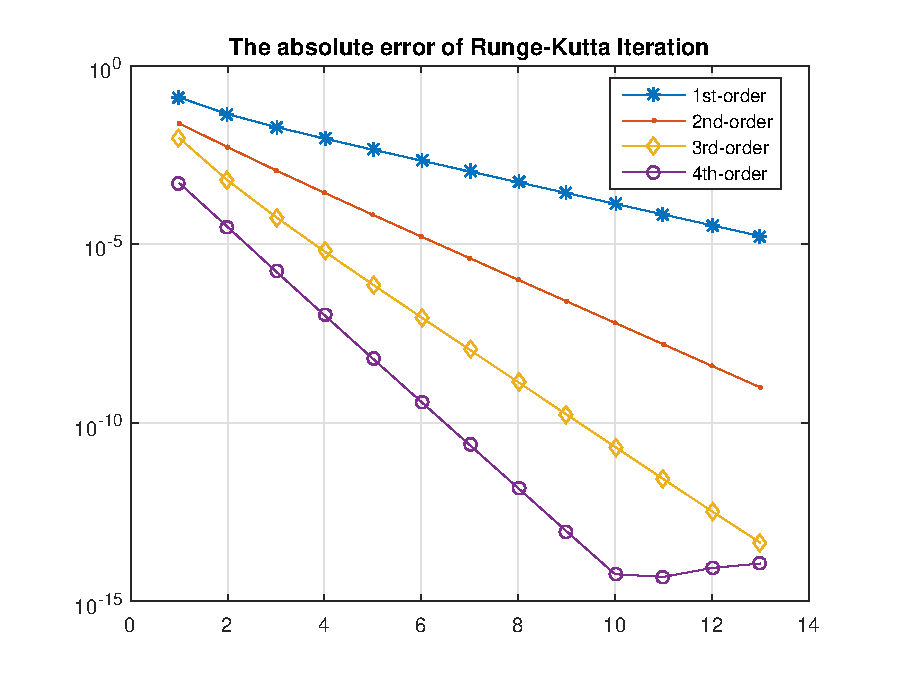
\includegraphics[width=15cm]{errorlist.eps}
\caption{The convergence order of 1-4 order format}
\label{convergence}
\end{figure}
}

\end{document}